\begin{SingleSpace}
\chapter{Linking the Climate and Thermal Phase Curve of 55 Cancri e}\label{ch:linking-climate-55cnce}
\vspace{0.5cm}
\chapterprecishere{``One face is forever sunlit, and one forever dark, and only the planet's slow liberation gives the twilight zone a semblance of seasons.''\par\raggedleft--- \textup{Stanley G. Weinbaum}, The Lotus Eaters}
\end{SingleSpace}
\vspace{0.5cm}




% 0 -- LEAD-IN PARAGRAPHS

%START ELEMENT

Now that I have introduced lava planets and 55 Cancri e in Chapter \ref{ch:lava-planets}, laid out a theory of their circulation in Chapters \ref{ch:wave-mean-flow} and X, and discussed the numerical model I used to simulate them in Chapter \ref{ch:sim-exofms}, I can move to the central question of this thesis. Namely, how to interpret the thermal emission phase curve of a tidally locked lava planet? The remaining chapters of my thesis will investigate this in increasing detail.

%FRAMING TEXT

The first phase curve of a Super-Earth was measured by \citet{demory201655cnce} using Spitzer observations of 55 Cancri e, following the measurement of transits in the visible \citep{winn201155cnce} and infrared
\citep{demory201155cnce}. This presented the first observation directly linked to the global circulation of a terrestrial planet outside our solar system. It provides an opportunity to test the theories and simulations of the atmospheric circulation of a tidally locked planet that have been shown previously in this thesis.

The thermal phase curve of 55 Cnc e presents the possibility of testing this picture of lava planets, and in particular to determine whether the phase curve demands
the presence of a thick noncondensible background atmosphere. In this paper, we use a general circulation
model (GCM) to model a range of hypothetical climates
for 55 Cnc e and reconstruct their thermal phase curve,
in order to test whether the observed phase curve is inconsistent with the presence of a thick atmosphere. We
explore which atmospheric compositions are compatible
with the phase curve. The results we have obtained
for 55 Cnc e will carry over readily to the interpretation of other lava planet phase curves when they become
available. The general utility of thermal phase curves in
determining characteristics of exoplanets and their atmospheres has been discussed in Selsis et al. (2011) and
Maurin et al. (2012).

The analysis in this paper builds on the results of
Cowan & Agol (2011), Menou (2012), and Komacek & Showman
(2016), who explored the effect of parameters such as the
mean molecular weight on the thermal phase curve of
Hot Jupiters via the radiative and advective timescales.
Koll & Abbot (2015) modelled the relation between
atmospheric properties and broadband thermal phase
curve for terrestrial planets in a regime (expected to be
appropriate to most tidally locked planets) with a significant phase curve amplitude, but very little hot-spot
offset. We have identified a regime which can support
both a notable amplitude and offset.


%SIGNPOSTS

Section 2 describes our model and explains the physical processes which it includes. Section 3 lays out the
current theory of global circulation on tidally locked
planets, where we discuss the key nondimensional parameters and situate 55 Cnc e in the space of circulation
regimes. We describe the results from our experiments
in Section 4, focusing on their temperature distributions
and simulated phase curves in comparison to the results
of Demory et al. (2016b). Further interpretation of the
results is provide in Section 5 and our principal findings
are summarized in Section 6.


%SUMMARISE CONCLUSIONS

Our best-fit clear-sky atmosphere has a surface pressure of 5 bar and a mean
molecular weight of 4.6 gmol−1
. This molecular weight
would support the hypothesis of an H2-rich atmosphere;
however, it is the observed hot-spot phase shift which
favours low molecular weight, underscoring the importance of accurate measurements of this quantity for future observations of 55 Cnc e and other lava planets.
A diagnostic estimate of cloud effects indicates that Na
clouds would not form in such an atmosphere, but that
SiO clouds could form on the night-side and bring the
modeled night-side brightness temperature more in line
with observations. Our results on the vertical structure
of the temperature pattern underscore the importance of
future measurements of spectrally resolved phase curves
for 55 Cnc e and other lava planets, which would provide
an important window into atmospheric composition and
dynamics.

In the next chapter, I will show how we coupled a more realistic radiative transfer scheme and a dynamic cloud model to Exo-FMS, in order to test the questions raised by this chapter.







%SECTION 1 -- PHASE CURVE
\section{Observations of 55 Cancri e}

%SUBSECTION --
\subsection*{55 Cancri e}


The first phase curve of a Super-Earth was measured by Demory et al. (2016b) using Spitzer observations of 55 Cancri e, following the measurement of
transits in the visible (Winn et al. 2011) and infrared
(Demory et al. 2011). 55 Cnc e is a Super-Earth discovered by McArthur et al. (2004) with mass 8.63 M⊕ and
radius 2.00 R⊕ in a close, tidally locked orbit with period
0.737 days.

%SUBSECTION --
\subsection*{Thermal Phase Curve}

The thermal phase curve has a large amplitude and an offset between its secondary eclipse and its
phase maximum. Demory et al. (2016b) used the curve
to reconstruct a temperature map with a maximum
hemisphere-averaged 4.5µm brightness temperature of
(2700 ± 270) K, day-night contrast of (1300 ± 670) K,
and a hot-spot shifted eastwards by (41 ± 12)◦

\begin{figure}
  \centering
  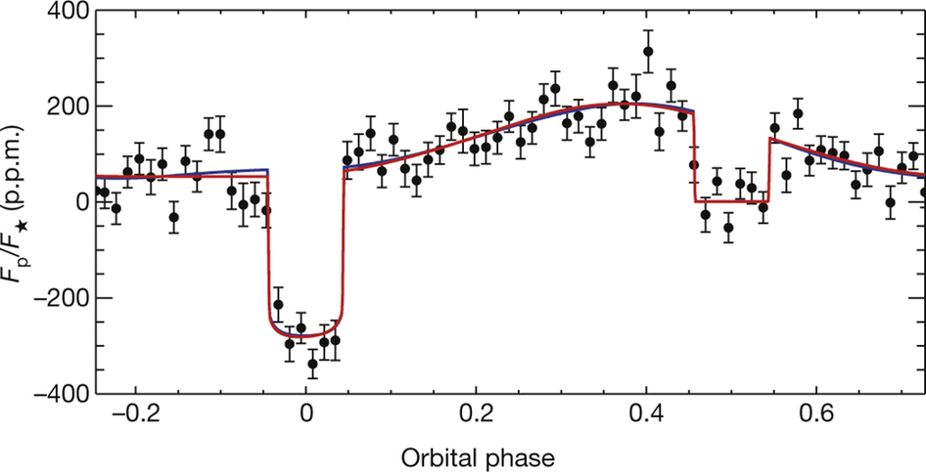
\includegraphics[width=0.66\textwidth]{figures/linking-climate-55cnce/demory-phase-curve.jpg}
  \caption{Phase curve.}
  \label{fig:demory-phase-curve}
\end{figure}

\begin{figure}
  \centering
  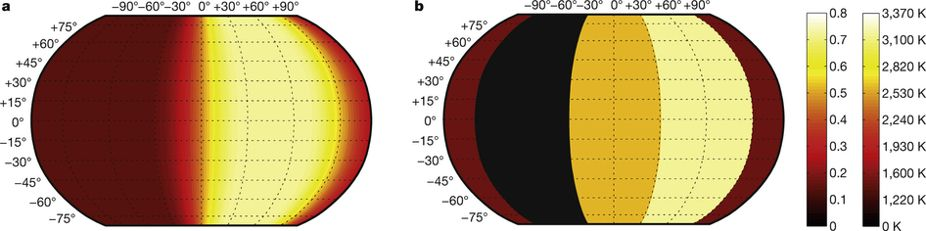
\includegraphics[width=1.0\textwidth]{figures/linking-climate-55cnce/demory-temperature-map.jpg}
  \caption{Temperature map.}
  \label{fig:demory-temperature-map}
\end{figure}

%SUBSECTION --
\subsection*{Possible Atmosphere}

55 Cnc e is a member of a class of planets known as
“lava planets” which are in such close orbits that they
are likely to be tide-locked and have a permanent dayside magma ocean. It has been argued that the atmospheres of such planets could consist of thin mineralvapour atmospheres outgassed from the magma ocean
(L´eger et al. 2011) (Castan & Menou 2011). Such thin
atmospheres, consisting of a few millibar or less surface
pressure, cannot transport much heat apart from possible lateral heat redistribution within the magma ocean,
so would yield a phase curve very similar to that of an
airless rocky planet with a very cold night-side such as
discussed by Maurin et al. (2012).

The transit depth spectra reported in Tsiaras et al.
(2016) require a thick H2-rich atmosphere. However,
Lammer et al. (2013) calculated that an H2 atmosphere
on 55 Cnc e would have a hydrodynamic escape rate
of up to 2.8 × 109 gs−1
. This implies that a 10 bar
atmosphere would be lost in less than one million years,
making it implausible that an H2-rich atmosphere could
be maintained on this planet. However, the study of
exoplanets has yielded up many objects that according
to previous conceptions should not exist, so in this paper
we will take the idea of an H2-rich atmosphere seriously,
and ask what features of the phase curve measured by
Demory et al. (2016b) are compatible with, or demand,
a low molecular weight atmosphere.
In order to focus on dynamical behavior in this initial
study, we make a number of simplifying assumptions regarding the radiative behavior of the atmosphere. First,
we assume the atmosphere to be transparent to incoming
stellar radiation, so that all of the shortwave radiation is
absorbed at the ground, leading to a deep day-side convective layer. This assumption is based on estimates of
the shortwave opacity of likely cloud-free atmospheres
of up to 10 bars. The addition of a small amount of
shortwave opacity would not change our results much,
so long as atmospheric absorption occurs near enough
the surface to drive a convective troposphere. Very
thick shortwave-opaque atmospheres could instead have
a deep radiative-equilibrium layer with a thin dynamically active layer near the top; we shall not consider
such atmospheres in the present paper.
In the infrared, the atmosphere is assumed to act as
a grey gas with specified optical thickness τ∞ and opacity κ. This is not inconsistent with the assumption of
an atmosphere largely transparent to incoming stellar
radiation, because 55 Cancri is a G star, with a relatively low proportion of its output in the near-IR. The
use of gray gas radiation for climate calculations is not
a serious source of inaccuracy as the circulation is primarily affected by the radiation scheme via the surface
temperature relative to the radiating temperature of the
planet. The optical thickness τ∞ can be tuned to match
the temperature that would be yielded by an assumed
real-gas atmosphere, so in this paper we use τ∞ primarily as a way to control surface temperature.
Non-grey radiative effects are taken into account when
we interpret the results in terms of the corresponding
Spitzer 4.5µm phase curve, in that we consider the emission from a range of different atmospheric levels and not
just the grey radiating level. This allows for the possibility that the atmospheric composition may support an
infrared window region near 4.5µm, allowing radiation
from deeper in the atmosphere, or a source of anomalous
opacity (e.g. clouds) there, forcing the radiating level to
be higher in the atmosphere.
The surface pressure determines the atmospheric mass
via the hydrostatic relation. For a given surface pressure and τ∞, atmospheric composition affects the climate through mean molecular weight and specific heat.
However, molar specific heat is only weakly dependent
Climate of 55 Cancri e 3
on composition, because it is primarily determined by
the number of active degrees of freedom. For example, at 2000K the molar specific heats of CO, N2 and H2
vary by no more than 3.4% relative to the mean value of
35.5 Jmol−1K−1
, with similar results for other common
diatomic gases. Triatomic gases have only a modestly
greater molar specific heat at 2000K, e.g. 60% higher
for CO2 or 46% higher for H2O. Therefore, the heat capacity of the atmosphere, which largely determines an
atmosphere’s ability to transport heat, is mostly determined by surface pressure and molecular weight. The
mean molecular weight also affects the speed of gravity
waves in the atmosphere, through its influence on the
gas constant. This speed determines the character of
many atmospheric waves which directly transport heat
and are implicated in the generation of super-rotating
low-latitude jets, which also transport heat. We present
our simulation results in terms of a range of H2-N2 mixtures, but they would apply accurately to any other diatomic mixture with the same molecular weight, and
with only moderate inaccuracy to triatomic-dominated
mixtures.


%SUBSECTION --
\subsection*{Atmospheric Circulation}

The measured phase curve of 55 Cnc e exhibits two
features that demand substantial horizontal heat transport. First, the hot spot of the planet is shifted 41◦
eastward relative to the substellar point. Second, the nightside temperature of the planet is quite high – on the
order of 1300K – demanding delivery of 1.6 × 105W/m2
of heating to maintain it. However, the day-night temperature difference is also large – on the order of 1300K
– which puts a limit on the efficiency of the heat transporting mechanism.
It has been suggested that the implied heat transport on 55 Cnc e might be carried by the magma ocean.
However, Kite et al. (2016) argued that a magma ocean
could not redistribute enough heat to affect a planet’s
measured phase curve. It is also conceivable that tidal
heating could contribute to maintaining the night-side
temperature. In this paper, we will focus on the question of whether atmospheric heat transport alone can
account for the phase curve, though we will offer some
remarks in Section 5 on problems with tidal heating as
an explanation of the night-side temperature.
The hot-spot phase shift and phase curve amplitude on tide-locked planets have been extensively studied in connection with interpretation of Hot Jupiter
phase curves. For sufficiently short period orbits,
the global circulation of such atmospheres is dominated by the effects of planetary scale equatorial
Rossby and Kelvin waves which drive a superrotating jet (Showman & Polvani (2011), Heng & Showman
(2015)). The circulation system transports heat eastwards around the equator, shifting the hot-spot from
the substellar point and warming the night-side of the
planet. The observed phase curve of 55 Cnc e poses
the particular challenge that its large 41◦ hot-spot shift
suggests strong heat redistribution, but its large 1300
K day-night difference suggests weak heat redistribution. The need to negotiate the tension between these
two requirements puts strong constraints on the kind of
atmosphere the planet can have.



%SUBSECTION --

%SECTION CONCLUSIONS


%SECTION 2 --
\section{Simulating a Lava Planet}

%SUBSECTION --

%SUBSECTION --

%SECTION CONCLUSIONS

%SECTION 3 --
\section{Simplified Scaling Theory}

Zhang

%SUBSECTION --

%SUBSECTION --

%SECTION CONCLUSIONS


%SECTION 3 --
\section{Idealised Simulations}

%SUBSECTION --
\subsection{Mean Molecular Weight}

%SUBSECTION --
\subsection{Surface Pressure}

%SUBSECTION --
\subsection{Optical Thickness}

%SUBSECTION --
\subsection{Vertical Structure}

%SUBSECTION --
\subsection{Phase Curves}

%SECTION CONCLUSIONS


%SECTION  --
\section{Discussion}

%SUBSECTION --
\subsection*{}


% %SECTION  --
% \section{Simulations with SOCRATES}
%
% %SUBSECTION --
% \subsection*{SOCRATES for Lava Planets}


%SECTION CONCLUSIONS


%CONCLUSIONS

%RESTATE SECTION CONCLUSIONS

%OPEN OUT CONCLUSIONS


% \bibliographystyle{unsrtnat}
% \bibliography{../references.bib}
